\begin{figure}[H]
\setlength{\linewidth}{\textwidth}
  \setlength{\hsize}{\textwidth}
    \centering
    % \subfigure[`\textit{pour milk}' from activity ``\textit{cereal}'']{\label{subfig:pmc2}
    % 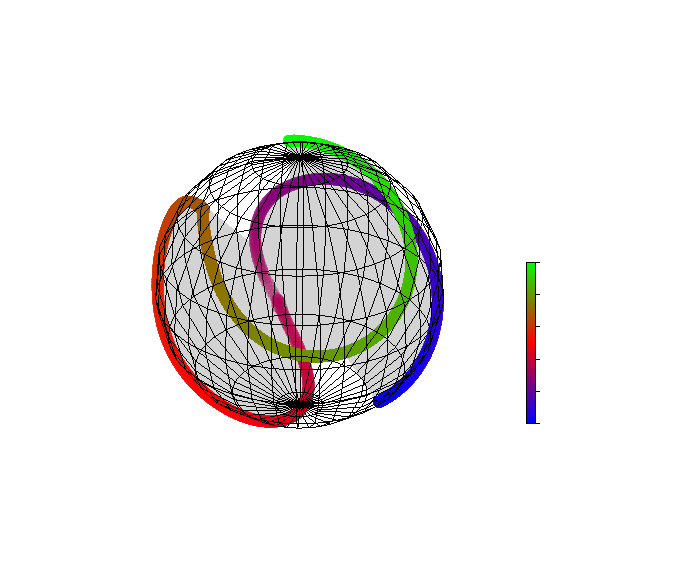
\includegraphics[width=0.55\linewidth]{chapters/ch-experiments/img/tc.pdf}
    % }
    \subfigure[`\textit{pour milk}' from activity ``\textit{cereal}'']{\label{subfig:pmc}
    \begin{overpic}[width=0.47\linewidth]{chapters/ch-experiments/img/tc.pdf}
        \put(93,3){\footnotesize 0.0}
        \put(93,9.5){\footnotesize 0.2}
        \put(93,16){\footnotesize 0.4}
        \put(93,22.5){\footnotesize 0.6}
        \put(93,29){\footnotesize 0.8}
        \put(92.9,35.5){\footnotesize 1.0}
        \put(80,5.5){ $c\!:$}
    \end{overpic}
    }\\
    \hfill
    \subfigure[`\textit{pour milk}' from activity ``\textit{cereal}'']{\label{subfig:pmc2}
    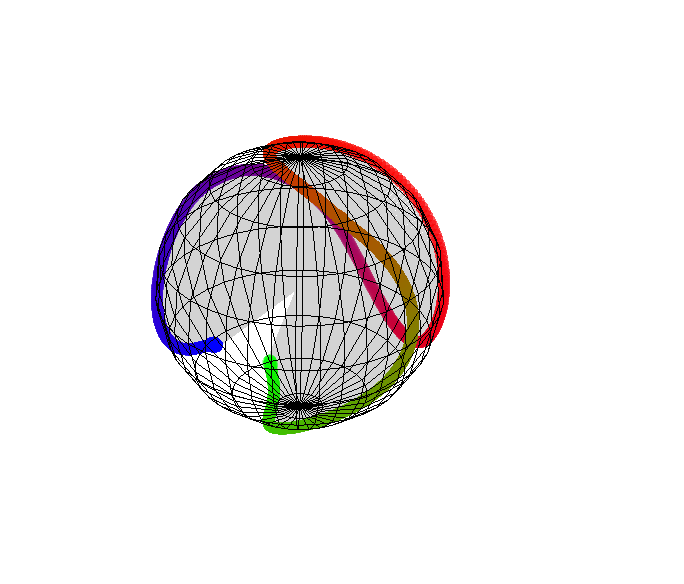
\includegraphics[width=0.33\linewidth]{chapters/ch-experiments/tex/pour_milk_cereal_2.pdf}
    }\hfill
    \subfigure[`\textit{take knife}' from activity ``\textit{juice}'']{\label{subfig:tkj}
    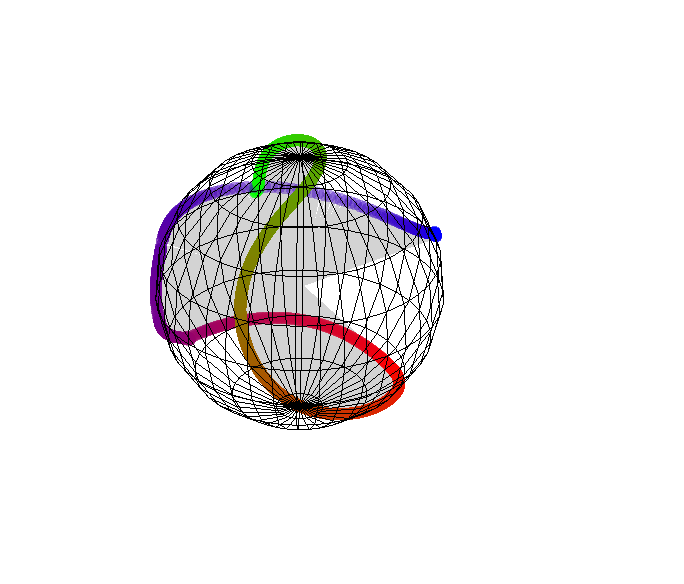
\includegraphics[width=0.33\linewidth]{chapters/ch-experiments/img/take_knife_juice.pdf}
    }\hfill
    \caption{T-SNE visualizations of generated action segments. %Every point in the sphere corresponds to a frame feature, and the continuity of these feature points demonstrates temporal coherence.
    }\label{fig:viz}
\end{figure}